% !TEX encoding = UTF-8 Unicode
\documentclass[a4paper]{article}

\usepackage{color}
\usepackage{url}
\usepackage[T2A]{fontenc} % enable Cyrillic fonts
\usepackage[utf8]{inputenc} % make weird characters work
\usepackage{graphicx}

\usepackage[english,serbian]{babel}
%\usepackage[english,serbianc]{babel} %ukljuciti babel sa ovim opcijama, umesto gornjim, ukoliko se koristi cirilica

\usepackage[unicode]{hyperref}
\hypersetup{colorlinks,citecolor=green,filecolor=green,linkcolor=blue,urlcolor=blue}

\usepackage{listings}

%\newtheorem{primer}{Пример}[section] %ćirilični primer
\newtheorem{primer}{Primer}[section]

\definecolor{mygreen}{rgb}{0,0.6,0}
\definecolor{mygray}{rgb}{0.5,0.5,0.5}
\definecolor{mymauve}{rgb}{0.58,0,0.82}

\lstset{ 
  backgroundcolor=\color{white},   % choose the background color; you must add \usepackage{color} or \usepackage{xcolor}; should come as last argument
  basicstyle=\scriptsize\ttfamily,        % the size of the fonts that are used for the code
  breakatwhitespace=false,         % sets if automatic breaks should only happen at whitespace
  breaklines=true,                 % sets automatic line breaking
  captionpos=b,                    % sets the caption-position to bottom
  commentstyle=\color{mygreen},    % comment style
  deletekeywords={...},            % if you want to delete keywords from the given language
  escapeinside={\%*}{*)},          % if you want to add LaTeX within your code
  extendedchars=true,              % lets you use non-ASCII characters; for 8-bits encodings only, does not work with UTF-8
  firstnumber=1000,                % start line enumeration with line 1000
  frame=single,	                   % adds a frame around the code
  keepspaces=true,                 % keeps spaces in text, useful for keeping indentation of code (possibly needs columns=flexible)
  keywordstyle=\color{blue},       % keyword style
  language=Python,                 % the language of the code
  morekeywords={*,...},            % if you want to add more keywords to the set
  numbers=left,                    % where to put the line-numbers; possible values are (none, left, right)
  numbersep=5pt,                   % how far the line-numbers are from the code
  numberstyle=\tiny\color{mygray}, % the style that is used for the line-numbers
  rulecolor=\color{black},         % if not set, the frame-color may be changed on line-breaks within not-black text (e.g. comments (green here))
  showspaces=false,                % show spaces everywhere adding particular underscores; it overrides 'showstringspaces'
  showstringspaces=false,          % underline spaces within strings only
  showtabs=false,                  % show tabs within strings adding particular underscores
  stepnumber=2,                    % the step between two line-numbers. If it's 1, each line will be numbered
  stringstyle=\color{mymauve},     % string literal style
  tabsize=2,	                   % sets default tabsize to 2 spaces
  title=\lstname                   % show the filename of files included with \lstinputlisting; also try caption instead of title
}

\begin{document}

\title{Klasifikacija skupa podataka \textit{Melanoma cell line}\\ \small{Seminarski rad u okviru kursa\\Istraživanje podataka 2\\ Matematički fakultet}}

\author{Nikola Dimić \\ mi15165 \\  dimic.nikola@gmail.com\\
mi15165@alas.matf.bg.ac.rs
}

\maketitle

\abstract{
Ovaj rad ima za cilj da najpre upozna čitaoca sa problemom klasifikacije ćelija u odnosu na otpornost na inhibitore koji se koriste u lečenju raka kože. Zatim će kroz primenu različitih klasifikacionih metoda i detaljnom analizom rezultata pokušati da otvori diskusiju o daljem korišćenju ovakvog tipa klasifikatora za istraživanja usmerena ka \textit{BRAF} inhibitorima i lečenju raka kože.
}
\tableofcontents

\newpage

\section{Uvod}
\label{sec:uvod}
U poslednjih nekoliko decenija oboljenje raka kože predstavlja jedno od najzastupljenijih vrsta kancera od kojih ljudi oboljevaju \cite{zastupljenost}. Ovo oboljenje najčešće se može prepisati prekomernom izlaganju ultra ljubičastom zračenju. Čak 230 hiljada ljudi godišnje oboli od ovog tipa raka po istraživanu ENCR (\textit{eng. European Network of Cancer Registries}) \cite{encr}. 

Brojna iztrazivanja bave se korišćenjem \textit{BRAF} inhibitora u svrhu lečenja ovog tipa karcinoma. \textit{BRAF} inhibitori suzbijaju sintezu ljudskog proteina B-Raf i na taj način onemogućavaju karcinom da se dalje širi \cite{braf}.

Kroz ovo istraživanje biće reči o klasifikaciji ćelija na one koje reaguju na tretman ove vrste i na one koje ne reaguju. Prvobitno kroz detaljnu analizu i obradu podataka skupa humanih ćelija \ref{analiza}, a zatim kroz primenu različitih metoda klasifikacije i analizu dobijenih rezultata biće tražen idealan klasifikacioni model kao i minimalan skup gena potreban za određivanje klase svake od ćelija \ref{klasifikacija}.

\section{Prikupljanje i obrada podataka}
\label{analiza}

Ulazne datoteke koje su korišćene u ovom radu predstavljaju podatke dobijene iz perifernih mononuklearnih ćelija (eng. \textit{Peripheral blood mononuclear cells, PBMCs}). Podaci predstavljaju rezultate istraživanja skupova humanih ćelija. Predstavljeni su sa dve datoteke u CSV (\textit{eng. Comma Seperated Values}) formatu u obliku ukrštene tabele
gde svaka datoteka ima 31222 reda,
od kojih prvi red sadrži redni broj ćelije za koju je istraživanje vršeno.

Broj redova je identičan u obe datoteke i svaki red je određen genom za koji se rezultati posmatraju.
Geni su predstavljeni u formatu hg38 što predstavlja oznaku da se radi o genu referentnog humanog genoma (\textit{eng. Genome Reference Consortium Human Reference 38)}.

Prva kolona sadrži redne brojeve ćelija za koje je istraživanje vršeno, a same vrednosti matrice predstavljaju broj traskripta gena u datoj ćeliji.
U tabeli \ref{table:1} predstavljen je deo tabele na osnovu kog se može zaključiti da je broj transkripta gena hg38\_A1BG u prvoj ćeliji jednak četiri. 
\begin{table}[h!]
\centering
\begin{tabular}{|c c c c c c|} 
 \hline
  & 1 & 2 & 3 & ... & 4305\\ [0.5ex] 
 \hline
 hg38\_A1BG & 4 & 0 & 0 & ... & 2 \\ 
 hg38\_A1BG-AS1 & 2 & 1 & 1 & ... & 2 \\
 hg38\_A2M & 0 & 0 & 0 & ... & 1 \\
 ... & ... & ... & ... & ... & .. \\
 hg38\_ZZEF1 & 2 & 2 & 0 & ... & 2 \\ [1ex] 
 \hline
\end{tabular}
\caption{Format ulaznih podataka}
\label{table:1}
\end{table}

Prva datodeka ima podatke o broju transkripata svakog od 31221 gena na 4305 ćelija dok je broj ćelija u drugoj datoteci 3950. 
Podaci su podeljeni tako da svi podaci koji se nalaze u jednoj datoteci pripadaju istoj klasi. 

\newpage
\subsection{Analiza podataka i klasa}

Pre klasifikacije podataka na osnovu datih tabela, neophodno je prvo podatke pripremiti i detaljno analizirati. 
U sklopu ovog istraživanja geni će biti posmatrani kao atributi klasifikacionog modela, pa je potrebno transponovati matrice koje se nalaze u obe datoteke.

Kako svi podaci unutar jedne datoteke pripadaju istoj klasi, potrebno je tu klasu dodati kao posebnu kolonu unutar matrica. Prva datoteka pripada klasi \textit{parental (BRAF inhibitor sensitive)} dok druga pripada \textit{BRAF inhibitor resistant}. \textit{BRAF} predstavlja ljudski gen koji enkodira protein \textit{B-Raf} \cite{braf}.
BRAF inhibitori, koji suzbijaju sintezu ovog proteina se koriste za lečenje raka kože. Međutim neretko se dešava da pacijenti postanu otporni na ovaj tretman. Taj slučaj predstavlja klasa \textit{BRAF inhibitor resistant} dok klasa \textit{parental (BRAF inhibitor sensitive)} predstavlja situaciju u kojoj ćelije reaguju na tretman \cite{therapy}.

Nakon dodavanja ovih klasa u datoteke matrice imaju redom 4305 i 3950 redova i 31222 kolona. U tabeli \ref{table:2} predstavljen je izgled matrice nakon dodavanja klase i transponovanja.

\begin{table}[h!]
\centering
\begin{tabular}{|c c c c c|} 
 \hline
  ć & hg38\_A1BG & ... & hg38\_ZZEF1 & Klasa \\ [0.5ex] 
 \hline
 1 & 1  & ... & 2 & BRAF inhibitor sensitive \\ 
 2 & 0  & ... & 3 & BRAF inhibitor sensitive \\
 3 & 1  & ... & 0 & BRAF inhibitor sensitive \\
 ... &  ... & ... & ... & BRAF inhibitor sensitive \\
 4305 & 5 & ... & 12 & BRAF inhibitor sensitive \\  [1ex] 
 \hline
\end{tabular}
\caption{Izgled matrice nakon dodate klase}
\label{table:2}
\end{table}

Kako su podacima dodeljene klase, potrebno ih je spojiti i tako se dobija matrica sa 8255 redova (ćelija) i 31222 kolone (gena). Nakon mešanja podataka kako bi se dobili podaci koji nisu poređani po klasama, dobijaju se podaci koji su predstavljeni tabelom \ref{table:3}.


\begin{table}[h!]
\centering
\begin{tabular}{|c c c c c|} 
 \hline
  ć & hg38\_A1BG & ... & hg38\_ZZEF1 & Klasa \\ [0.5ex] 
 \hline
 1 & 1  & ... & 2 & BRAF inhibitor sensitive \\ 
 2 & 0  & ... & 3 & BRAF inhibitor resistant \\
 3 & 7  & ... & 7 & BRAF inhibitor sensitive \\
 ... &  ... & ... & ... & BRAF inhibitor sensitive \\
 8255 & 1 & ... & 22 & BRAF inhibitor resistant \\  [1ex] 
 \hline
\end{tabular}
\caption{Izgled matrice nakon spajanja tabela}
\label{table:3}
\end{table}
\subsection{Eliminacija nula}
\label{elnula}

Na osnovu analize podataka može se zaključiti da kolone koje imaju sve nula vrednosti ne mogu značajno uticati na dalje istraživanje. Kako bi se redukovala dimenzija skupa podataka i tako ubrzali procesi klasifikacije, ovakve kolone odnosno geni se izbacuju iz skupa razmatranja. Kako su podaci kao predmet istraživanja podeljeni u dve datoteke nula kolone se mogu eliminisati na dva načina:

\begin{itemize}
  \item \textbf{Slab uslov za eliminaciju nula (Unija)} \newline
    Ukoliko kolona odnosno gen ima sve nula vrednosti u skupu podataka sa klasom \textit{BRAF inhibitor sensitive} \textbf{i} u skupu podataka sa klasom \textit{ BRAF inhibitor resistant} ta kolona se izbacuje iz sjedinjenog skupa podataka. Kolone koje su značajne za istraživanje predstavljaju \textbf{uniju} nenula kolona oba skupa podataka.
  \item \textbf{Jak uslov za eliminaciju nula (Presek)} \newline
    Ukoliko kolona odnosno gen ima sve nula vrednosti u skupu podataka sa klasom \textit{BRAF inhibitor sensitive} \textbf{ili} u skupu podataka sa klasom \textit{ BRAF inhibitor resistant} ta kolona se izbacuje iz sjedinjenog skupa podataka. Kolone koje su značajne za istraživanje predstavljaju \textbf{presek} nenula kolona oba skupa podataka.
\end{itemize}

Koristeći obe tehnike značajno se smanjuje broj relevantnih podataka unutar sjedinjene tabele pa je dimenzija matrice nakon eliminacija nula smanjena sa 31221. kolone na 21848. kolona u slučaju korišćenja slabog uslova eliminacije (unije), odnosno na 18753. kolone u slučaju korišćenja jakog uslova eliminacije tj. preseka. 

U nastavku rada biće razmatrani rezultati korišćenja oba uslova eliminacije pa će klasifikacione metode biti testirane na dva različita skupa podataka.

\subsection{Obrada nedostajućih vrednosti}
Kako je potrebno izvršiti različite tehnike klasifikacije koje ne rade sa nedostajućim vrednostima neophodno je naći i obraditi takve vrednosti ako postoje. Nakon izvršene provere, zaključuje se da ovaj skup nema nepostojećih vrednosti pa dalja obrada nije potrebna.

\subsection{Obrada elemenata van granica}
\label{outlier}

Nakon analize podataka i njihovog značenja, dolazi se do zaključka da posmatranje elemenata van granica u skupu ćelija odnosno redova matrice podataka nije od značaja. Kako svaka ćelija u u nekoj koloni nema ni jedan ili ima veći broj transkripata gena, eliminacijom elemenata van granica eliminisali bismo sve podatke. Iz navedenog razloga, fokus ovog rada u ovom kontekstu biće nalaženje elemenata van granica u skupu kolona.

Za pronalaženje kolona koje su više ili manje relevantne za istraživanje korišćena z vrednost implementirana pomoću funkcije \textbf{z-score} iz biblioteke \textbf{scipy.stats} programskog jezika \textit{Python}. Ova ocena računa se po sledećoj formuli:

\[ 
z = \frac{(x-\mu)}{\sigma}
\]

Eliminacijom nula kolona izbačene su kolone koje ne sadrže dovoljno informacija kako bi bile relevantne za istraživanje pa primenom ove statističke metode nije dobijen ni jedan element van donje granice \cite{zscore}.

Nasuprot tome, čak 1748 kolona predstavljaju elemente van gornje granice. Kako ove kolone sadrže značajno više informacija nego ostale, u nastavku rada biće posvećeno dosta pažnje analizi ovih podataka. 
Uporednim testiranjem klasifikacionih metoda na ovim i na celokupnim podacima, testira se hipoteza da se na osnovu malog skupa podataka od samo 1748 gena može dobiti ista ili slična klasifikaciona moć kao i na osnovu celokupnog skupa gena.

\newpage

\section{Klasifikacija}
\label{klasifikacija}

U ovom segmentu rada biće predstavljene različite metode klasifikacije kao i rezultati dobijeni tim metodama. Sve klasifikacione metode primenjene su kako na skup dobijen korišćenjem jakog, tako i na skup dobijen korišćenjem slabog uslova eliminacije nula. Ovi skupovi će respektivno biti referisani dalje u tekstu kao skup unije i skup preseka.

Za proces same klasifikacije neophodno je razdvojiti podatke na test i trening skup kako bi bio kreiran klasifikacioni model koji nije preprilagođen datim podacima. 
Odnos test i trening skupa u odnosu na podatke je 40-60 (za test skup je odvojeno 40\% podataka dok je za trening skup odvojeno 60\% podataka).

\subsection{Skup unije i preseka}

Primenom svih klasifikacionih metoda na skupove unije i preseka dolazi se do zaključka da se u oba slučaja dobijaju jako slični rezultati. Kako bi ovaj rad bio koncizan i bez prekomernog ponavljanja, u okviru ovog dela biće predstavljeni i analizirani rezultati klasifikacije skupa unije, dok će rezultati klasifikacije skupa preseka biti predstavljeni tabelom u dodatku \ref{dodatak}. Skup unije ima 8255 redova, odnosno 21848 kolona.

\subsubsection{Klasifikacija metodom stabla odlučivanja}
\label{dt}

Klasifikacija metodom stabla odlučivanja primenjena je korišćenjem klasifikatora \textit{DecisionTreeClassifier} iz biblioteke \textbf{sklearn} za programski jezik \textit{Python}. Ovaj klasifikator koristi optimizovani \textit{CART (eng. Classification And Regression Tree)} algoritam kako bi kreirao stablo odlučivanja za posmatran skup podataka.

U okviru ovog istraživanja primenjene su različite mere nečistoće za izračunavanje dobiti pa su testirane metode klasifikacije koristeći ginijev indeks kao i entropije. 

Informaciona dobit za čvor m za ginijev indeks izračunava se sledećom formulom:

$$H(X_m) = \sum_{k}(p(m|k) * ( 1 - p(m|k) ))$$

Analogno, informaciona dobit za čvor m u slučaju korišćenja entropije kao mere nečistoće izračunava se formulom:

$$H(X_m) = -\sum_{k}(p(m|k) * log( p(m|k) ))$$

Korisno je naći stablo sa minimalnom dubinom koje daje zadovoljavajuće rezultate pa je stablo potrebno potkresati.
Posmatrane vrednosti za potkresivanje tj za maksimalnu dubinu stabla odlučivanja su 3, 4 i 6. Radi uporedne analize tačnosti klasifikacionog modela biće posmatrana i opcija bez potkresivanja stabla. Dobijeni rezultati tačnosti pomenutih modela primenjenog na test i trening skup podataka prikazani su tabelom \ref{table:4}.  Takođe, biće posvećena pažnja i tome koliko je vremena potrebno za kreiranje samog modela podataka \cite{classification}.

\begin{table}[h!]
\centering
\begin{tabular}{|c c c c|} 
 \hline
  potkresivanje & trening skup & test skup & vreme 
  \\ [0.5ex] 
 \hline
 bez potkresivanja & 100 \% & 98.4 \% & 60s \\
 6 & 99.6 \% & 98.4 \% & 32s \\
 4 & 99.1 \% & 98.3 \% & 59s \\
 3 & 98.3 \% & 98.3 \% & 50s \\ [1ex] 
 \hline
\end{tabular}
\caption{Preciznost klasifikacionog modela u zavisnosti od dubine stabla}
\label{table:4}
\end{table}

Korišćenje entropije kao mere nečistoće daje veoma slične rezultate, pa će na dalje biti razmatrani 
samo rezultati dobijeni korišćenjem ginijevog indeksa. 
Na osnovu prikazanih rezultata može se zaključiti da ova metoda klasifikacije daje odlične rezultate čak i za malu dubinu stabla. Posmatranjem grafika generisanih programom za obradu podataka, dolazi se do zaključka da prvih par podela odlično dele prostor pretrage, što se detaljnije vidi na slici \ref{fig:slikastablo}. 

Vreme konstruisanja modela je slično za sve vrednosti i varira u intervalu od 30 do 60 sekundi ukoliko se izvršava na \textit{2.7 GHz Intel Core i5} procesoru.

\begin{figure}[h!]
\centering
 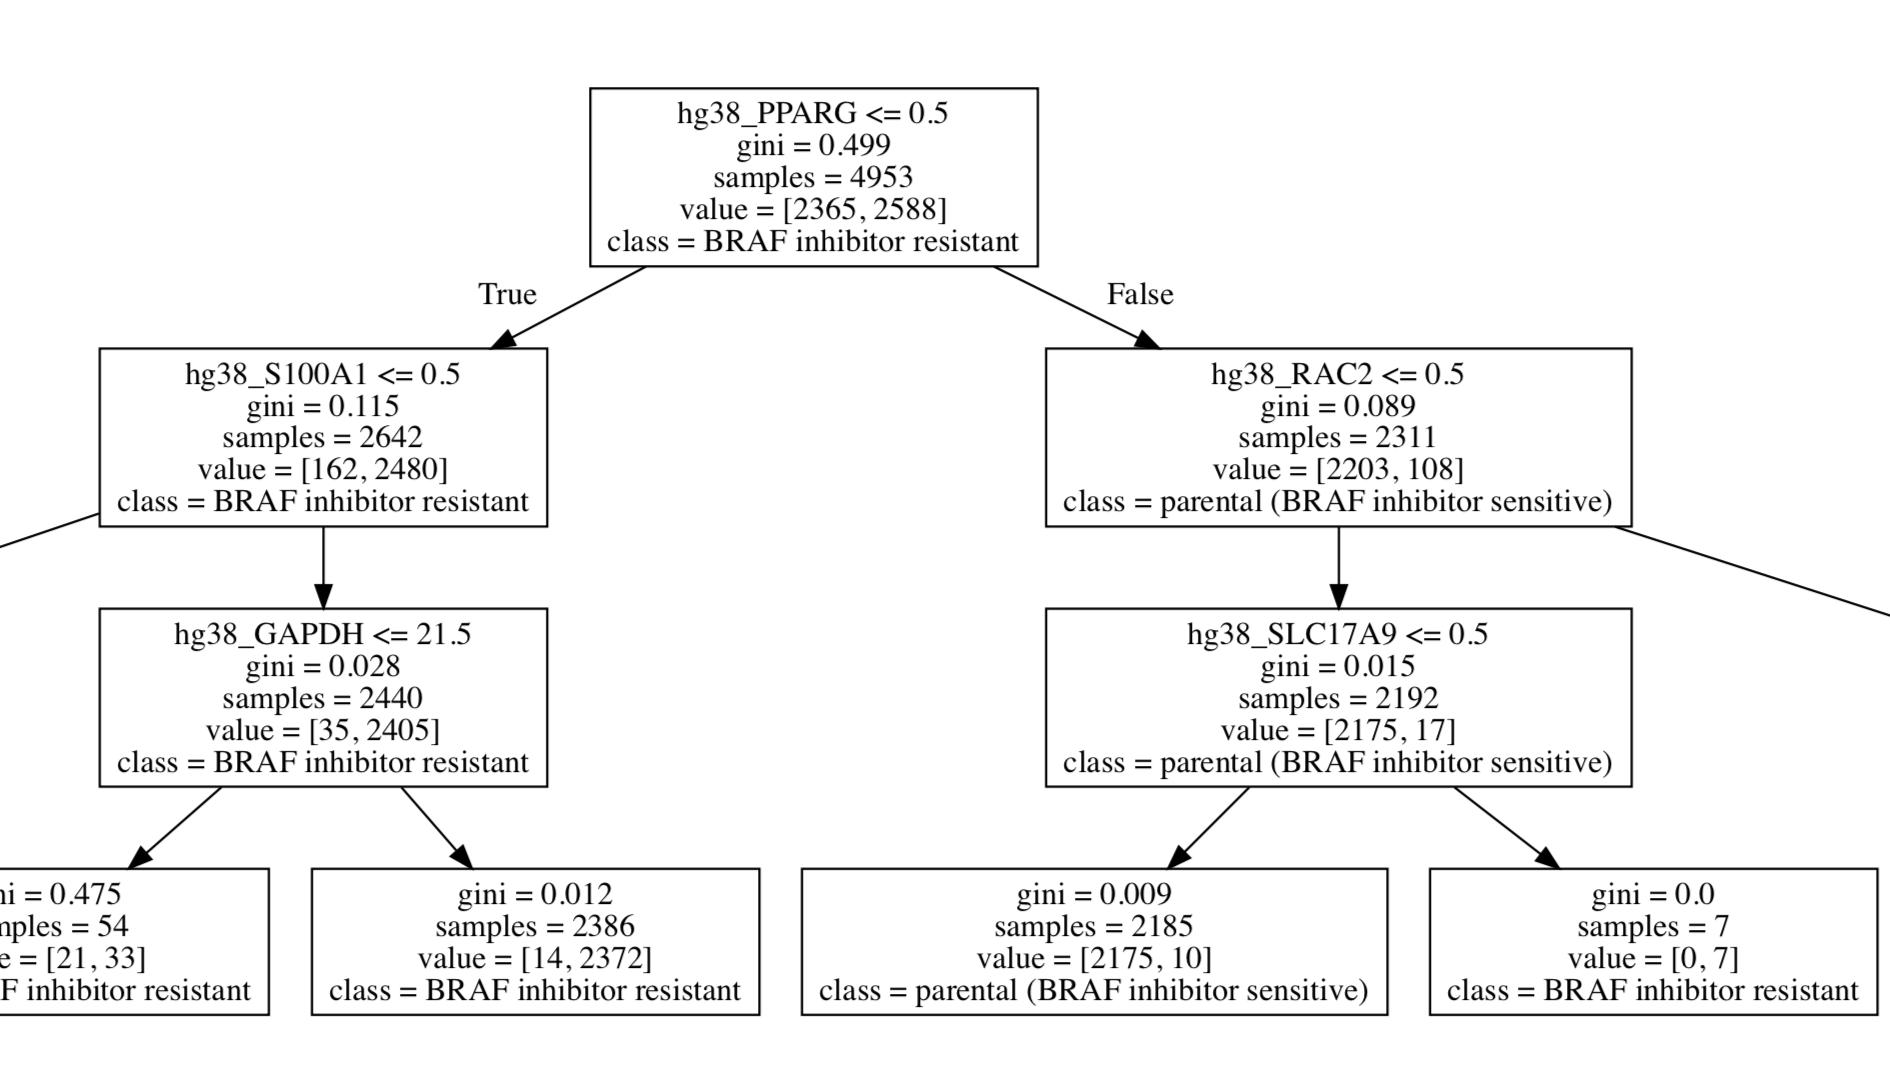
\includegraphics[width=1\textwidth]{slikastablo.png}
 \caption{Deo stabla odlučivanja sa maksimalnom dubinom 3}
 \label{fig:slikastablo}
\end{figure}

Posmatranjem slika stabala u sva 4 posmatrana slučaja može se zaključiti da je gen hg38\_PPARG jako bitan za zaključivanje klase datih elemenata.
Detaljnije analize mogu se sprovesti posmatranjem matrica konfuzije koje su predstavlene u tabeli \ref{table:5}. Svaka matrica konfuzije data je u obliku :

\begin{table}[h!]
\centering
\begin{tabular}{|c c|}
  \hline
  TP & FN \\
  FP & TN  \\
 \hline
\end{tabular}
\caption{Oblik matrice konfuzije}
\label{table:0}
\end{table}

\begin{itemize}
  \item TP \textit{(eng. True positives)} - broj elemenata koji pripadaju prvoj klasi  tj \textit{BRAF inhibitor sensitive} i koji su tako klasifikovani.
  \item FN \textit{(eng. False negatives)} - broj elemenata koji pripadaju klasi \textit{BRAF inhibitor sensitive} a koji su klasifikovani suprotno.
  \item FP \textit{(eng. False positives)} - broj elemenata koji ne pripadaju \textit{BRAF inhibitor sensitive} klasi a koji su klasifikovani kao da joj pripadaju.
  \item TN \textit{(eng. True negatives)} - broj elemenata koji ne pripadaju \textit{BRAF inhibitor sensitive} klasi a koji tako i klasifikovani.
\end{itemize}

\begin{table}[h!]
\centering
\begin{tabular}{|c c c|} 
  \hline
  dubina stabla & \multicolumn{2}{c|}{matrica konfuzije} \\ [0.5ex] 
  \hline
  bez potkresivanja & 1563 & 22 \\
     & 32 & 1685  \\
  \hline
  6 & 1562 & 23 \\
     & 32 & 1685  \\
  \hline
  4 & 1562 & 23 \\
     & 30 & 1687  \\
  \hline
  3 & 1554 & 31 \\
     & 25 & 1692  \\
 [1ex] 
 \hline
\end{tabular}
\caption{Stablo odlučivanja - matrice konfuzije test skupa}
\label{table:5}
\end{table}

Posmatrajući matricu konfuzije na test skupu, primećuje se da se FN vrednosti uvećavaju sa smanjenjem maksimalne dubine stabla dok se FP vrednosti smanjuju. Ipak, ukupan zbir ovih vrednosti ne varira mnogo, pa je hipoteza da se i sa većim potkresivanjem stabla dobija jednako precizan model potvrđena \cite{classification}.

\subsubsection{Klasifikacija metodom k najbližih suseda}
\label{ksusedasekcija}


Klasifikacija metodom k najbližih suseda primenjena je korišćenjem klasifikatora \textit{KNeighborsClassifier} iz biblioteke \textbf{sklearn} za programski jezik \textit{Python}. Ovaj klasifikator koristi  \textit{Lopta stablo (eng. Ball Tree)} , Kd stablo (eng. Kd Tree) ili algoritam grube sile za nalaženje k najbližih suseda.

U okviru ovog istraživanja korišćene su sve varijante ovog algoritma. U zavisnosti od implementacije klasifikatora tj odabira algoritma dobijaju se rezultati prikazani u tabeli \ref{table:algknn}.

\begin{table}[h!]
\centering
\begin{tabular}{|c c c c|} 
 \hline
  algoritam & trening skup & test skup & vreme 
  \\ [0.5ex] 
 \hline
 kd stablo & 99.2 \% & 98.6 \% & 15 min \\
 lopta stablo & 99.4 \% & 98.6 \% & 15 min \\
 algoritam grube sile & 99.2 \% & 98.6 \% & 1.5 min \\
 \hline
\end{tabular}
\caption{Preciznost klasifikacionog modela u zavisnosti od odabira algoritma}
\label{table:algknn}
\end{table}

Preciznost samog klasifikacionog ne varira mnogo u zavisnosti algoritma, ali je brzina kreiranja modela umnogome zavisi od odabira algoritma. Kako algoritam grube sile na \textit{2.7 GHz Intel Core i5} procesoru konstruiše klasifikacioni model čak 10 puta brže nego drugi algoritmi u daljim analizama biće korišćen ovaj algoritam.

Uporednom analizom matrica konfuzije koje se dobijaju prilikom testiranja klasifikacionih modela koji se razlikuju po parametru k, može se zaključiti koji je broj suseda idealan za posmatrani problem. Parametar k predstavlja upravo broj najbližih suseda na osnovu čijih klasa se zaključuje klasa posmatranog podatka. Ovaj odnos prikazan je u tabeli \ref{table:knnconfusion}. Matrica konfuzije prikazana je u istom formatu kao što je opisano u sekciji \ref{dt}.

\begin{table}[h!]
\centering
\begin{tabular}{|c c c|} 
  \hline
  broj suseda & \multicolumn{2}{c|}{matrica konfuzije} \\ [0.5ex] 
  \hline
  3 & 1570 & 26 \\
     & 8 & 1698  \\
  \hline
  5 & 1567 & 29 \\
     & 9 & 1697  \\
  \hline
  10 & 1571 & 25 \\
     & 12 & 1694  \\
  \hline
  16 & 1564 & 32 \\
     & 12 & 1694  \\
 [1ex] 
 \hline
\end{tabular}
\caption{KNN - Matrice konfuzije test skupova u zavisnosti od k}
\label{table:knnconfusion}
\end{table}

Kako vreme izvršavanja u slučaju različitog broja suseda značajno ne varira može se zaključiti da je idealan broj posmatranih suseda 3. Broj pogrešno klasifikovanih podataka ogleda se na sporednoj dijagonali pa je u ovom slučaju taj broj najmanji \cite{classification}.

\subsubsection{Klasifikacija metodom
potpornih vektora}
\label{potVektor}

Mašine sa potpornim vektorima predstavljaju skup metoda za klasifikaciju, regresiju i pronalaženje nedostajućih vrednosti. U sklopu ovog istraživanja za potrebe klasifikacije korišćen je klasifikator \textit{SVC} iz biblioteke \textbf{sklearn} za programski jezik \textit{Python}. Ovaj klasifikator koristi  \textit{C-SVC} algoritam. U okviru ovog istraživanja korišćene su različite kernel funkcije koje su definisane u tabeli \ref{table:kerneli}. 

Parametri $\gamma$ , $d$ i $r$ su redom određeni parametrima klasifikatora. Pokazalo da za $\gamma$, podrazumevana vrednost $1/|Y|$ gde je $|Y|$ broj kolona odnosno gena skupa podataka, daje odlične rezultate. Slično se može zaključiti za vrednosti 3 i 0 za parametre $d$ i $r$ respektivno.



\begin{table}[h!]
\centering
\begin{tabular}{|c c|} 
 \hline
  naziv kernela & formula\\ [0.5ex] 
 \hline
 polinomijalni & $(\gamma <x, x_1> + r )^{d}$\\ 
 RBF kernel & $exp(- \gamma * ||x - x_1||^{2})$\\
 sigmoidni & $tanh(\gamma <x, x_1> + r )$\\
 \hline
\end{tabular}
\caption{Korišćene definicije kernel funkcija}
\label{table:kerneli}
\end{table}

Kako se metod potpornih vektora zasniva na ideji 
nalaženja razdvajajuće hiper ravni tako da su svi 
podaci date klase sa iste strane ravni, može se 
očekivati da će za pažljivo odabranu kernel 
funckiju koja odgovara skalarnom proizvodu u višedimenzionom prostoru, ova tehnika dati dobre rezultate \cite{classification}. Za gore navedene kernel funkcije dobijeni su rezutati tačnosti klasifikacije dati u tabeli \ref{table:svmtacnost}.

\begin{table}[h!]
\centering
\begin{tabular}{|c c c c|} 
 \hline
  naziv kernela & trening skup & test skup & vreme 
  \\ [0.5ex] 
 \hline
 polinomijalni & 100 \% & 99.3 \% & 1.6 min \\
 RBF kernel & 100 \% & 72.6 \% & 35 min \\
 sigmoidni & 46.9 \% & 48.6 \% & 40 min \\ [1ex] 
 \hline
\end{tabular}
\caption{Preciznost klasifikacionog modela u zavisnosti od kernel funkcije}
\label{table:svmtacnost}
\end{table}

 Sigmoidna kernel funkcija se najčešće koristi za 
 klasifikaciju slika pa je jasno da u slučaju ovog problema daje jako loše rezultate. Sa druge starane, u slučaju primene RBF kernel funkcije
 dolazi do preprilagođavanja pa model daje odlične rezultate na trening skupu ali na test skupu ima 
 znatno lošije rezultate. Ova tvrdnja može se potkrepiti i analizom matrice konfuzije \ref{table:rbf}. 

\begin{table}[h!]
\centering
\begin{tabular}{|c c|}
  \hline
  1556 & 9 \\
  914 & 823  \\
 \hline
\end{tabular}
\caption{RBF kernel funkcija - matrica konfuzije test skupa}
\label{table:rbf}
\end{table}

Može se primetiti da je broj \textit{FP} vrednosti, odnosno broj elemenata koji ne pripadaju klasi a klasifikovani su kao da joj pripadaju, jako veliki pa možemo zaključiti da ova kernel funkcija nije adekvatna za klasifikaciju posmatranog skupa podataka.

\begin{table}[h!]
\centering
\begin{tabular}{|c c|}
  \hline
  1553 & 12 \\
  9 & 1728  \\
 \hline
\end{tabular}
\caption{Polinomijalna kernel funkcija - matrica konfuzije test skupa}
\label{table:poli}
\end{table}


Nasuprot tome, prilikom korišćenja polinomijalne kernel funkcije dobijaju se odlični rezultati kako za trening tako i za test skup. Posmatrajući matricu konfuzije datu u tabeli \ref{table:poli} zaključujemo da do preprilagođavanja nije došlo i da je klasifikacioni model zaista najprecizniji od svih prethodno posmatranih metoda.

\subsubsection{Klasifikacija asambl metodama}
\label{asambl}

Primenom različitih klasifikacionih metoda traži se onaj koji daje najbolje rezultate odnosno onaj gde je greška klasifikacionog modela najmanja. Vođene ovom idejom, metode asambla kombinuju različite modele za predviđanje kako bi minimizovali grešku klasifikacije. Metode asambla testirane su kroz sledeća dva predstavnika.

\begin{itemize}
\item \textbf{\textit{Bagging}}

\textit{Bagging} predstavlja asambl tehniku koja iz ulaznih podataka uzima uzorke sa ponavljanjem i kreira klasifikator za svaki od njih. Za potrebe ovog istraživanja korišćen je klasifikator \textit{BaggingClassifier} iz biblioteke \textbf{sklearn} za programski jezik \textit{Python}. Podešavanjem broja klasifikatora pokazalo se da korišćenjem 5 klasifikatora dobija model koji ima zadovoljavajuću klasifikacionu moć kako u smislu preciznosti tako i u smislu vremena potrebnog za kreiranje i testiranje modela.

Klasifikatori koji se kreiraju na svakom od 
uzoraka su podešavani i testirani za metodu 
potpornih vektora, metodu k najbližih suseda kao 
i metodu kreiranja stabla odlučivanja. Dobijeni 
su rezultati prikazani tabelom \ref{table:bagging}.


\begin{table}[h!]
\centering
\begin{tabular}{|c c c c|} 
 \hline
  klasifikator & trening skup & test skup & vreme 
  \\ [0.5ex] 
 \hline
 slablo odlučivanja & 99.91 \% &  99.09 \% & 3.7 min \\
 k najbližih suseda & 99.49 \% &  99.06 \% & 14.9 min \\
 SVM &  99.87 \% &  99.57 \% & 10.2 min \\
 \hline
\end{tabular}
\caption{Preciznost bagging metoda u zavisnosti od klasifikatora}
\label{table:bagging}
\end{table}

Metoda potpornih vektora \textit{(eng. SVM)} 
davala je najbolje rezultate dosad pa je slično i u slučaju korišćenja više klasifikatora. Stoga 
analizom matrice konfuzije dobijenog 
klasifikatora primenjenog na test skup prikazane tabelom \ref{table:bagkonf}, možemo zaključiti da je model gotovo perfektan jer su pogrešno klasifikovani slogovi svedeni na miniumum.

\begin{table}[h!]
\centering
\begin{tabular}{|c c|}
  \hline
  1590 & 9 \\
  5 & 1698  \\
 \hline
\end{tabular}
\caption{\textit{Bagging} - Matrica konfuzije test skupa}
\label{table:bagkonf}
\end{table}

Međutim, kako se dobijeni rezultat ne razlikuje od onog dobijenog samo jednim klasifikatorom, ova tehnika nije optimalna kako je za kreiranje modela potrebno mnogo više vremena.


\item \textbf{\textit{Boosting}}

\textit{Boosting} predstavlja asambl tehniku koja prvobitno kreira slab klasifikator, a zatim slogovima dodeljuje težine i kroz iteracije adaptira klasifikator u odnosu na težine. U okviru ovog istraživanja korišćen je AdaBoost klasifikator koji adaptivno podešava težine, konkretnije klasifikator iz biblioteke \textbf{sklearn} - \textit{AdaBoostClassifier}.

Za početni klasifikator koji se podešava u odnosu na dodeljene težine izabrani su klasifikatori dobijeni metodom potpornih vektora i stabla odlučivanja i rezultati su upoređeni kako bi se našao onaj za koji je novonastali klasifikator najbolji. Nije iznenađenje da SVM klasifikator daje za nijansu bolje rezultate ali je potrebno mnogo duže da se klasifikator kreira. Zato će u nastavku biti korišćen klasifikator slabla odlučivanja. 

Podešavanjem brzine učenja klasifikatora dobijaju se rezultati prikazani tabelom \ref{table:boosttable}
pa je zaključak da za sve vrednosti bliske 1.0 klasifikator daje odlične rezultate.

\begin{table}[h!]
\centering
\begin{tabular}{|c c c c|} 
 \hline
  brzina učenja & trening skup & test skup & vreme 
  \\ [0.5ex] 
 \hline
 0.5 &  100 \% &  99.81 \% & 2.23 min \\
 0.7 &  100 \% &  99.91 \% & 2.21 min \\
 0.9 &  100 \% &  99.91 \% & 2.25 min \\
 1 & 100 \% & 99.87 \% & 2.24 min \\
 1.2 & 100 \% &  99.81 \% & 2.41 min \\

 \hline
\end{tabular}
\caption{Preciznost boosting metoda u zavisnosti od brzine učenja}
\label{table:boosttable}
\end{table}

Analizom matrice konfuzije u tabeli \ref{table:boostkonf} dolazi se do zaključka da je ovom metodom postignut najbolji rezultat odnosno najtačniji klasifikator od svih prethodno analiziranih.

\begin{table}[h!]
\centering
\begin{tabular}{|c c|}
  \hline
  1571 & 3 \\
  3 & 1725  \\
 \hline
\end{tabular}
\caption{\textit{Boosting} - Matrica konfuzije test skupa}
\label{table:boostkonf}
\end{table}
\newpage

\end{itemize}
\subsection{Skup elemenata van granica}

Elementi van granica u zadatom skupu predstavljaju gene koji sadrže neuobičajeno više ili manje informacija u odnosu na ostale kao što je pomenuto u odeljku \ref{outlier}. Kako u skupu nema donjih elemenata van granica svi posmatrani elementi su oni koji sadrže značajne informacije. Postavlja se pitanje, da li je moguće da se na osnovu samo ovih gena dobije ista ili slična klasifikaciona moć kao i korišćenjem celog skupa podataka. 

Ta hipoteza proverena je korišćenjem onih klasifikacionih modela koji su se najbolje pokazali pri obradi celog klasfikacionog skupa. Posmatrani skup je redukovan na 1748 gena što je manje od 10\% celokupnog skupa.

\subsubsection{Klasifikacija metodom stabla odlučivanja}

Primenom istog klasifikatora kao u sekciji \ref{dt}, uz korišćenje ginijevog indeksa kao mere nečistoće, kreira se stablo odlučivanja čija je maksimalna dubina 4. Ovaj model tačno klasifikuje trening podatke u 98.9\% slučaja, dok kod test podataka taj broj iznosi 98\%. Kako je skup znatno manji, za pravljenje klasifikacionog modela, i matrica konfuzije bilo je potrebno svega 2.34 sekunde pri izvršavanju na \textit{2.7 GHz Intel Core i5} procesoru.

\begin{table}[h!]
\centering
\begin{tabular}{|c c|}
  \hline
  1565 & 25 \\
  41 & 1671  \\
 \hline
\end{tabular}
\caption{Stablo odlučivanja - matrica konfuzije test skupa}
\label{table:soo}
\end{table}
 
Posmatrajući matricu konfuzije prikazanu tabelom \ref{table:soo} zaključuje se da je broj elemenata na sporednoj dijagonali porastao tj da je klasifikator lošiji u odnosu na onaj koji je koristio ceo skup podataka, ali da je ta razlika jako mala, pa se s obzirom na brzinu izvršavanja ovaj klasifikator može uzeti kao relevantan u daljem istraživanju.

\subsubsection{Klasifikacija metodom k najbližih suseda}

Analizom rezultata dobijenih na celom klasifikacionom skupu i algoritama koji koriste metodu k najbližih suseda dolazi se do zaključka da je za ovu vrstu klasifikacije najpogodnije koristiti algoritam grube sile što je detaljno opisano u sekciji \ref{ksusedasekcija}. Ukoliko se parametar k, tj broj posmatranih suseda postavi na 3, dobija se klasifikacioni model sa tačnošću od 99.5\% na trening odnosno 98.9\% na test skupu. 

Ovaj klasifikacioni model je zapravo još tačniji od onog koji koristi ceo skup podataka upravo iz razloga što su nepotrebni podaci uklonjeni pa se razdaljine između sličnih ćelija izračunavaju sa većom preciznošću.

\begin{table}[h!]
\centering
\begin{tabular}{|c c|}
  \hline
  1567 & 23 \\
  11 & 1701  \\
 \hline
\end{tabular}
\caption{KNN - matrica konfuzije test skupa}
\label{table:knnoo}
\end{table}

Brzina kreiranja samog modela je takođe značajno bolja pa je na  \textit{2.7 GHz Intel Core i5} procesoru za to potrebno 7.8 sekunde. Matrica konfuzije prikazana je tabelom \ref{table:knnoo}.

\subsubsection{Klasifikacija metodom
potpornih vektora}

Mašine sa potpornim vektorima pokazale su se kao 
najefektivniji metod za klasifikaciju celokupnog 
skupa ukoliko se koristi polinomijalna kernel 
funkcija kao što je detaljno opisano u sekciji 
\ref{potVektor}. Primenivši isti klasifikator na redukovani skup od 1748 gena kreira se model čiju klasifikacionu moć treba uporediti sa prethodno navedenim modelom. 

Kao što se pokazalo da klasifikacija metodom k najbližih suseda daje malo bolje rezultate kada je skup redukovan zbog veće tačnosti izračunavanja razdaljine izmedju jedinki odnosno ćelija, tako se i u slučaju klasifikacije metodom potpornih vektora dobijaju odlični rezultati zbog tačnije pozicije svakog podatka u n dimezionom prostoru.

Naime klasifikovanje test skupa uradjeno je sa tačnošću od čak 99.57 \% što je najbolji rezultat na test skupu. Posmatrajući matricu konfuzije test skupa prikazanu tabelom \ref{table:redPot} možemo primetiti da su vrednosti na sporednoj dijagonali najniže i da je samo 14 jedinki klasifikovano netačno.

\begin{table}[h!]
\centering
\begin{tabular}{|c c|}
  \hline
  1615 & 4 \\
  10 & 1673  \\
 \hline
\end{tabular}
\caption{SVM - matrica konfuzije test skupa}
\label{table:redPot}
\end{table}

Kao i za sve operacije nad skupom sa redukovanim brojem kolona brzina kreiranja i izvršavanja modela nad podacima je znatno poboljšana. Iako tačniji od klasifikatora koji koristi metodu k najbližih suseda, SVM klasifikator je malo sporiji pa je \textit{2.7 GHz Intel Core i5} procesoru za klasifikaciju bilo potrebno 4.8 sekunde.


\subsubsection{Klasifikacija asambl metodama}
\label{asamblskr}

Asambl metode koje koriste više klasifikatora kako bi kreirale model koji je značajno precizniji dale su odlične rezultate na celokupnom skupu kao što je detaljno opisano u sekciji \ref{asambl}. Primenom istih metoda \textit{bagging} i \textit{boosting} koristeći parametre koji su se pokazali kao efektivni na celokupnom skupu potrebno je testirati hipotezu da će ova tehnika i na skupu sa manjim brojem gena dati slične rezultate.

\begin{itemize}
\item \textbf{\textit{Bagging}}

Korišćenjem metoda potpornih vektora za kreiranje 5 klasifikatora nad uzorcima i zatim primenom \textit{boosting} algoritma dobija se klasifikator sa tačnošću od 99.9 \% na trening, odnosno 99.2  \% na test skupu.

\item \textbf{\textit{Boosting}}

Korišćenjem \textit{boosting} algoritma gde je početni klasifikator koji se podešava upravo stablo odlučivanja dobija se tačnost od čak 99.87 \% na test skupu skupu. Matrica konfuzije prikazana tabelom \ref{table:asamblKonf}
samo je potvrda da je od 3302 reda koja se nalaze u skupu za testiranje pogrešno klasifikovano samo 4 što je definitivno najbolji rezultat dosadašnjih analiza. 



\begin{table}[h!]
\centering
\begin{tabular}{|c c|}
  \hline
  1590 & 1 \\
  3 & 1708  \\
 \hline
\end{tabular}
\caption{\textit{Boosting} - Matrica konfuzije test skupa}
\label{table:asamblKonf}
\end{table}

Uzevši u obzir i brzinu izvršavanja i kreiranja modela koja iznosi 18.4 sekunde na \textit{2.7 GHz Intel Core i5} procesoru stiče se utisak da iako više puta sporiji od prethodnih klasifikatora za redukovan skup ovaj klasifikator daje sasvim zadovoljavajuće rezultate.


\end{itemize}

\section{Zaključak}
\label{sec:zakljucak}

Kroz osvrt na različite vrste klasifikacije i njihovu primenu došlo se do zaključka da se ćelije unutar ljudskog genoma na osnovu malog skupa gena mogu klasifikovati do skoro savršene tačnosti. To se može postići naprednijim asambl metodama ili metodama potpornih vektora pa ovo istraživanje predstavlja mali korak ka multidisciplinarnosti i mogućoj realnoj primeni ovakve vrste klasifikacionih metoda u medicini.

Detaljnijom analizom podataka i primenom još naprednijih klasifikacionih metoda ovaj model može da se unapredi pa ovaj rad predstavlja odličan uvod za dalja istraživanja o značaju pojedinih gena u cilju određivanja otpornosti ćelija na različite tretmane za lečenje karcinoma. 

\addcontentsline{toc}{section}{Literatura}
\appendix
\bibliography{seminarski} 
\bibliographystyle{plain}

\newpage
\appendix
\section{Dodatak}
\label{dodatak}

U narednoj tabeli prikazana je preciznost klasifikatora ukoliko je korišćen skup preseka o kome je bilo reči u sekciji \ref{elnula}. Slike drveta odlučivanja mogu se naći priložene uz ovaj rad.


\begin{table}[h!]
\centering
\begin{tabular}{|c c c c c|} 
 \hline
  klasifikator & varijanta & trening skup  & test skup & vreme 
  \\ [0.5ex] 
 \hline
 slablo odlučivanja & potkresivanje - 6 nivoa & 99.69 \% &  98.24 \% & 25s \\
 slablo odlučivanja & potkresivanje - 4 nivoa & 99.24 \% &  98.27 \% & 21s \\
  slablo odlučivanja & potkresivanje - 3 nivoa & 98.41 \% &  98.00 \% & 20s \\
 slablo odlučivanja & bez potkresivanja & 100 \% &  98.15 \% & 32s \\
 K najbližih suseda & broj suseda - 3 & 99.51 \% &  99.06 \% & 1.39 min \\
 K najbližih suseda & broj suseda - 5 & 99.35 \% &  98.90 \% & 1.32 min \\
 K najbližih suseda & broj suseda - 10 & 99.03 \% &  98.54 \% & 1.23 min \\
 K najbližih suseda & broj suseda - 15 & 98.71 \% &  98.40 \% & 1.26 min \\
 SVM & kernel funkcija - RBF & 100 \% &  71.32 \% & 33 min \\
 SVM & kernel funkcija - sigmoid & 51.88 \% &  51.05 \% & 45 min \\
 SVM & kernel funkcija - polinom. & 99.97 \% &  99.57 \% & 1.18 min \\
 
bagging & 3 klasifikatora & 99.61 \% &  98.63 \% & 2.5 min \\
bagging & 5 klasifikatora & 99.79 \% &  98.78 \% & 4.2 min \\
bagging & 7 klasifikatora & 99.89 \% &  98.94 \% & 5.2 min \\
bagging & 10 klasifikatora & 99.87 \% &  98.78 \% & 7.7 min \\

bagging & svm klasifikator & 99.91 \% &  99.57 \% & 16.1 min \\
bagging & stablo odlučivanja & 99.75 \% &  98.78 \% & 3.86 min\\
bagging & knn klasifikator & 99.43 \% &  99.27 \% & 8.83 min \\

boosting & brzina učenja - 0.5 & 100 \% &  99.87 \% & 2.6 min \\
boosting & brzina učenja - 0.7 & 100 \% &  99.90 \% & 2.2 min \\
boosting & brzina učenja - 0.9 & 100 \% &  99.90 \% & 2.1 min \\
boosting & brzina učenja - 1.0 & 100 \% &  99.93 \% & 2.5 min \\
boosting & brzina učenja - 1.2 & 100 \% &  99.87 \% & 2.7 min \\
 \hline
\end{tabular}
\caption{Preciznost klasifikacionih metoda na presek skupu}
\label{table:dodatak}
\end{table}


\end{document}
